\section{Background Introduction}
In the age of Internet dating, there are more romantic options than fish in the well. Many daters believe that having more options means they're more likely to find the right person for they while many daters find that less romantic options may lead to better outcomes without much anxiety. In another view, when faced with a myriad of choices, the pleasure at the prospect of more options is canceled out by the anticipated loss of making a wrong choice.  Actually, research has found that speed daters often choose their partners based on their looks. But when faced with fewer options, daters are likely to take the time to reflect on a person's deeper qualities. That suggests that in order to evaluate the qualities that matter -- which, for most people, are things like a partner’s honesty, his dependability, her sense of humor—going deeper in search but not wider is necessary.\par
Considering these phenomena, some feasible and scientific algorithms or methods can be applied to recommend appropriate partners for people want to find boy friend or girl friend.

\section{The Description of Problem}   
\subsection{Problem One: Online Dating Matches  }  
The request of problem one is concise: Create an objective quantitative algorithm or set of algorithms to complete online dating matches by few options. There are two steps we can follow:

\begin{enumerate}
	\item \textbf{Unsupervised Learning}: Since the data set of human beings can be very huge, we can filter all the human sample data to several classes, which is irrelevant to the attributes of data. This process can be regarded as unsupervised learning, so K-means algorithm can be considered. 
	\item \textbf{Supervised Learning}: According to data on few options, some objective functions and certain constraints could be set up. Aimming at the online dating matches, some algorithms in personalization recommendation such as K-Nearest Neighbor, Matrix Decomposition Recommender System, User-Based Collaborative Filtering, Model-Based Collaborative Filtering and Psychology-Based Recommendation can all be used in our dating matches models. This process can be regarded as supervised learning.
\end{enumerate}

\subsection{Problem Two:  More Suitable Estimate of An Ideally Sized Choice Set}                 
The goal of this problem is to give a more suitable estimate of an ideally sized choice set in the development of "Top 20 Recommended Daters" list established from problem one. Some Manual analysis can be done on the information of the top 20 daters from more angles and finally a best daters visualized report of eight persons can be generated and presented to the user to see his or her ideal daters with variety and depth consideration. 


\subsection{Problem Three: Information Forms Design and Effect Analysis Study}
This problem consists of two parts:
\begin{quote}
\begin{itemize}
	\item Design the information forms.
	\item Study the relationship between forms design and success rate of online dating. 
\end{itemize}
\end{quote}
\par
For the design of forms, apart from some necessary information that every user must give, different kinds of questions can be designed to different users according to their unique personality traits. Besides, different size, style of forms can all be adopted to gather detailed information from users indirectly.\par
For the relationship study, a relational matrix between quantitative analysis of forms and the success rate of online dating can be established and then this problem is transferred to an regression problem which can be solved in quite a lot ways such as Linear Regression, Logistic Regression, Polynomial Regression, Stepwise Regression or even Support Vector Machine.

\subsection{Problem Four:  Non-Technical News Release }
 Problem four requires to write a one-page non-technical News Release describing the algorithms used, the results, and the website designed, which is based on the first three problems. With the limitation of one page, some refinement and streamlined form of expressions must be considered.  

\section{Terminology Explained in Model \cite{1}}      
\begin{itemize}        
	\item Unsupervised Learning: A branch of machine learning that learns from test data that has not been labeled, classified or categorized. Instead of responding to feedback, unsupervised learning identifies commonalities in the data and reacts based on the presence or absence of such commonalities in each new piece of data. 
	\item Supervised learning: The machine learning task of learning a function that maps an input to an output based on example input-output pairs. A supervised learning algorithm analyzes the training data and produces an inferred function, which can be used for mapping new examples.
	\item Loss Function and Objective Function: In mathematical optimization, statistics, econometrics, decision theory, machine learning and computational neuroscience, a loss function or cost function is a function that maps an event or values of one or more variables onto a real number intuitively representing some "cost" associated with the event. An optimization problem seeks to minimize a loss function. An objective function is either a loss function or its negative (in specific domains, variously called a reward function, a profit function, a utility function, a fitness function, etc.), in which case it is to be maximized. 

\end{itemize}


\section{Assumptions}
1. Assume that all the data needed in models, algorithms or forms design are available in reality.

2. All data we want to collect are selected based on whether is useful for correct daters recommendation without privacy considerations. 

3. Assume that data from users are all true and reliable and no need of noise elimination.

4. No small probability or random events in the recommendation system, such as world war and economic crisis.

5. Assume that personality traits of users do not change significantly over time.

\section{Symbols and Definitions}

\begin{center}
	\begin{tabular}{|p{80pt}|c|p{80pt}|}
		\hline
		\makebox[0.15\textwidth][c]{\textbf{symbol}}	& \makebox[0.1\textwidth][c]{\textbf{Meanings}} \\ \hline
	    $\mathbf{Scores_{i,j}}$        &  score of j\_th person through i\_th person's eyes         \\ \hline
		m       & number of male users           \\ \hline
		w       & number of female users  \\ \hline
		u       & number of users, $u=m+w$    \\ \hline
	    N  & the top N recommended daters    \\ \hline
	    onum     &   number of options selected in a specific situation \\ \hline
	   \textbf{ User\_Item} &  a matrix with shape(u,), column number is optional. \\ &
	    $User_i$\_$Item_j$ means the value of i\_th user on j\_th item \\ \hline
	    \textbf{Top}    &    a matrix storing information of recommended daters.\\ \hline
	\end{tabular}
\end{center}
%\begin{figure}[!htbp]                                       
%	\centering
%	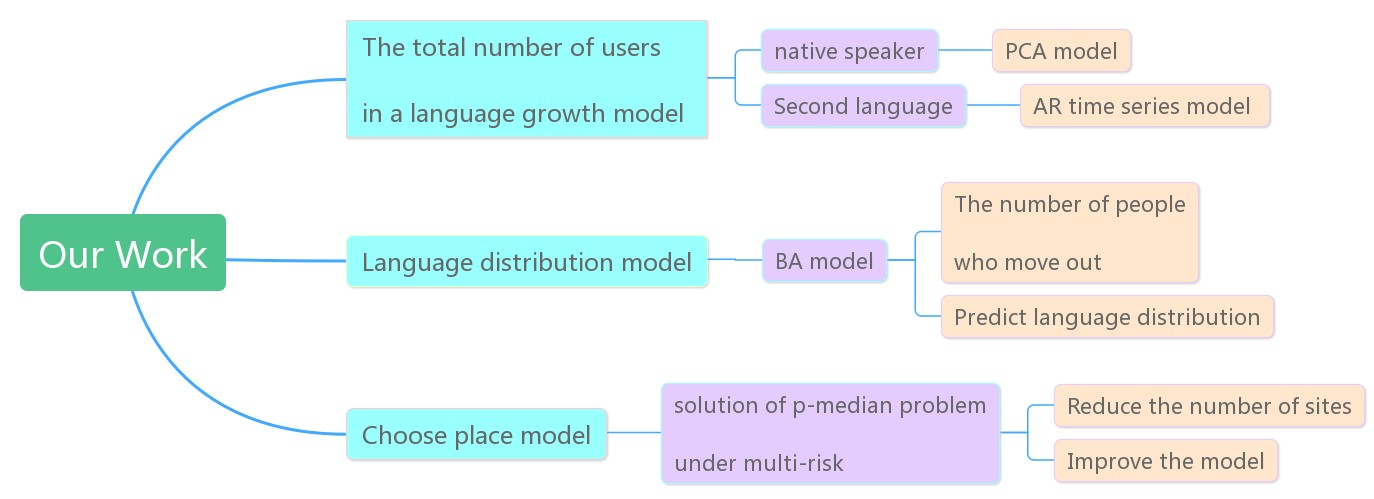
\includegraphics[width = .8\textwidth]{ourwork.jpg}      
%	\caption{Flow Chart}                          
%	\label{ourwork}                                      
%\end{figure}
%\begin{figure}[!htbp]                                      
%	\centering
%	\includegraphics[width = .8\textwidth]{introduction.jpg}      
%	\caption{The Distribution of Various Language}                                  
%	\label{introduction}                                           
%\end{figure}
\section{Problem Solutions with Model Foundation}  
\subsection{Solution for Problem One} 
\subsubsection{General Idea}                              

Since the main task of this problem is to complete online dating matches, we can regard it as a recommendation system problem. We name the system \textbf{Perfect Dater Partner Online Recommendation System}. The core of this system is the dater match algorithm which can analyse the information of users inputting online and quickly recommend an ideally sized object choice set to users. \par
Nowadays, there are many mature recommendation algorithms in online shopping, online movies which can recommend perfectly appropriate goods. But when it comes to recommend daters, things become serious and more complex. 
\indent
\paragraph{Object Matrix}
For evaluating which person is a ideal object for a user called $U1$, we can construct a two-dimensional square matrix named \textbf{Scores}. The shape of \textbf{Scores} is $(u,u)$, we have to obtain the final Scores between every pair of users including each pair of two men and two women. This is a general solution which can calculate all the probability of two person regardless of their sex. In reality, we may divide the user data set to several parts according to their sexual orientation, in which the shape could be $(m,w), (w,m), (m,m), (w,w), (w,u), (m,u)$. But for universality and simplification, we only consider the \textbf{Scores} matrix with shape $(u,u)$ as our evaluation matrix. The element $\mathbf{Scores_{i,j}}$ means the score of j\_th person through i\_th person's eyes. Through comparing and quickly sorting(Quick Sort Algorithm) the Scores in one row, the top \textbf{N} daters of $U1$ are easily founded. 

\paragraph{Few Options}
According to the meaning of problem and for simplification, use few options as the inputs of algorithms. Due to different options needed by different algorithms, the detailed options will be shown in individual model.

\paragraph{Similarity Measurement \label{sm}}
A significant aspect is the way to measure the gap of two people which could be references of constructing objective function. The distance(or similarity) measurement methods we can use are very abundant\cite{2}:\\
\begin{tabular}{p{0.3\linewidth}p{0.4\linewidth}p{0.3\linewidth}}
	\textbullet \ \textbf{ Euclidean Distance} & \textbullet \  Manhattan Distance  & \textbullet \ Chebyshev Distance \\
	\textbullet \ Minkowski Distance & \textbullet \   Mahalanobis Distance & \textbullet \  \textbf{Cosine Distance}\\
	\textbullet \ Information Entropy & \textbullet \ Hamming Distance & \textbullet \ Jaccard Distance \\
	\textbullet \ 	Correlation Distance & \textbullet \ Standardized Euclidean Distance
\end{tabular}
For example, Euclidean Distance can be presented as followed:
\begin{equation}
{\textrm{ED}}(u_1,u_2) = \sqrt {{{(u{_{11}} - u_{21})}^2} + {{(u_{12} - u_{22})}^2} + ... + {{(u{_{1onum}} - u{_{2onum}})}^2}}
\end{equation}
$u_1, u_2$ mean two users to be evaluated; $u_{1i}$ means the score of $u_1$ on the i\_th option; $onum$ means the number of options selected.\\
Another example, Cosine Distance:
\begin{equation}
\cos ({u_1},{u_2}) = \frac{{\sum\limits_{i = 1}^{onum} {{u_1}_i{u_2}_i} }}{{\sqrt {\sum\limits_{i = 1}^{onum} {{u_1}_i^2} } \sqrt {\sum\limits_{i = 1}^{onum} {{u_2}{{_i}^2}} } }}
\end{equation}
All the distance measurement methods can be used to calculate the similarity of two persons. Training and testing work are needed as for which method is the best idea. \par
Our groups have tried to use some suitable algorithms based on daters recommendation, just see them in next several sections.

\subsubsection{Model 1: K-means}

This algorithm is only used for processing big data set. It can divide the whole data set into K clusters according to their global attributes distribution. The similar samples will be classified into the same cluster so that daters can be easier to find in the cluster they belong. 

The core of this algorithm is the way to measure the gap and initialize the positions of K centroids. For gap measurement, any similarity measurement method discussed in \ref{sm} are accepted. For the initialization of centroids, the following formula can be adopted:
\begin{equation}
	 centroidSet[i,j] = min(j)+(max(j)-min(j))*random(0,1)
\end{equation}
$centroidSet[i,j]$ means the value of j\_th option in i\_th centroid vector; $min(j)$ and $max(j)$ means the minimum and maximum value under the j\_th option; $random(0,1)$ means a random number between 0 and 1.

\paragraph{Inputs} A numerical matrix: \textbf{User\_Item}. The number of rows is u. The number of columns could be very large. Each value shows a user's evaluation or attribute about a item. A item could be any goods, things and any personal information.  
\paragraph{Outputs} A two-dimensional matrix named \textbf{User\_Class} with shape (u,2). The first column represents the ID of user and the second presents the class number to which this user belongs. Each user has a unique class number.

\paragraph{Application}
Since we do not have any big data set, an example program of K-means applied in \textbf{UCI Iris} data set is shown in appendix \ref{apA}. It is based on python language version 3.6.6 and run on jupyter notebook(a kind of Integrated Development Environment). We use the Euclidean Distance as the measurement of the gap between two samples and assign the K parameter to 3. Finally, the data set is divided to 3 clusters.

\paragraph{Strength and Weakness}
\subparagraph{Strength}
\begin{itemize}
	\item It's a unsupervised learning process without consideration of options.
	\item Can easily and scientifically divide the data set into K sets, which is helpful for processing big data sets.
	\item No need of complex operations. The calculation is simple and clear.
	\item Time complexity(O(uKt), t is the iteration number) and space complexity(O(u*onum)) is nearly O(n), which is acceptable.
\end{itemize}
\subparagraph{Weakness}
\begin{itemize}
	\item Can not know the meaning of each cluster, need further assessment. 
	\item The result and effect is difficult to assess.
	\item Need to set a appropriate parameter K value and find a suitable similarity measurement method.
\end{itemize}

\subsubsection{Model 2: KNN}
The full name of KNN is K-nearest neighbor. By using a similarity measurement method in \ref{sm}, for each user, KNN algorithm can recommend the top K daters who are well-matched with him or her. The distance smaller, the similarity degree bigger. To be clear, the goal here is not to classify a user to which class, but just to get the K-nearest neighbor as the Top K daters.
\paragraph{Few Options} The options here must have a characteristic that the difference value of a option between two users smaller, the matching degree of the two users higher. For example, the options could be goods and the values could represent how much users like the goods. Besides, personal information like educational background, age, height and weight can also be included. 

\paragraph{Inputs}  A numerical matrix with shape(u, onum): \textbf{User\_Item}. onum is the number of few options selected. Each value shows a user's evaluation or attribute about an option.  

\paragraph{Output} A two dimensional matrix with shape(u,2*K): \textbf{Top}. K columns store top K ID of matched daters and the other K columns store the scores. It could be a result of daters recommendation. By the way, it is a optimization compared to the \textbf{Scores} while \textbf{Top} needs fewer space.

\paragraph{Application}
Still based on data set \textbf{UCI Iris}, we run an example program using KNN algorithm. The full codes are shown in appendix \ref{apB}. We still use the Euclidean Distance as the measurement of the gap between two samples and assign the K parameter to 3. Since the KNN is a supervised learning process, we can calculate the accuracy and finally get an average accuracy rate 95.64\%. The results can be seen in figure \ref{1}.
\begin{figure}[h]
	%\small
	\centering
	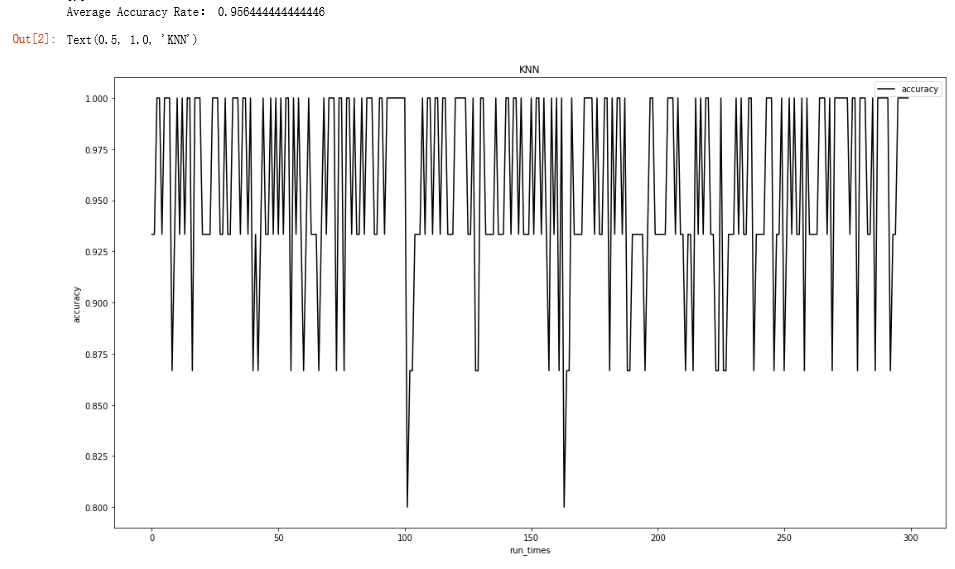
\includegraphics[width=19cm]{m3.png}
	\caption{Results of Accuracy Rate with 300 run times}  \label{1}
\end{figure}
\newpage
\paragraph{Strength and Weakness}
\subparagraph{Strength}
\begin{itemize}
	\item Scientifically recommend the best k daters to each user, making it easy to choose friend from huge boundless sea of faces.
	\item It is a supervised learning process, which is very targeted and specific.
	
\end{itemize}
\subparagraph{Weakness}
\begin{itemize}
	\item Do not separate the affection from user A to user B and affection from user B to user A, which should be different since different person have different request, so constraints need to be introduced.
	\item With time complexity O(n*n), this algorithm may be a little slow.
	\item Options related needs to be filtered carefully by staff.
	
\end{itemize}

\subsubsection{Other Models }
Due to the limitation on time and data, we decide to just give a brief description of other models or algorithms that can be used in our daters recommendation system.

\begin{itemize}
	\item Collaborative Filtering Recommendation:
	Collaborative filtering is a method of making automatic predictions(filtering) about the interests of a user by collecting preferences or taste information from many users(collaborating). The underlying assumption of the collaborative filtering approach is that if a person A has the same opinion as a person B on an issue, A is more likely to have B's opinion on a different issue than that of a randomly chosen person. There are three mainly recommendation of collaborative filtering: Matrix factorization, Bayesian Belief Nets CF Models, Probabilistic Factor models.
	\item Content-based Recommendation
	\item Association Rule-based Recommendation
	\item Utility-based Recommendation
	\item Knowledge-based Recommendatio
	\item Hybrid Recommendation
\end{itemize}
%\subparagraph{Matrix factorization}
%
%\subparagraph{Bayesian Belief Nets CF Models}
%
%\subparagraph{Probabilistic Factor models}
%
%
%\paragraph{Content-based Recommendation}
%
%\paragraph{Association Rule-based Recommendation}
%
%\paragraph{Utility-based Recommendation}
%
%\paragraph{Knowledge-based Recommendation}
%
%\paragraph{Hybrid Recommendation}

\subsubsection{Models Optimization }

\begin{enumerate}
	\item Let's go back to the original established goal matrix \textbf{Scores}. When calculating the top K daters we just use comparison and Quick Sort Algorithm in each row of the matrix. For different objects, they may score differently from each other which means $Scores_{i,j} != Score_{j,i}$. So as for a user, we can add each $Score_{j,i}$ to each $Scores_{i,j}$ as a final matching degree, then do sorting algorithm on the sum matrix. In this way, the feelings of both sides are taken into account.
	\item Since before the K-means require one user only belong to one cluster, now we can divide all the options into many aspects and do K-means on every aspect. In this way, data sets are divided into many different hierarchical clusters according to different classification criteria and we know which cluster is relevant to which aspect. A user can be classified to more than one class and KNN algorithm can be done in every aspect, which means our recommendation is more specific and targeted.
	
\end{enumerate}

%\begin{figure}[!htbp]              
%	\centering
%	\subfloat[ACF and PACF]{                               
%		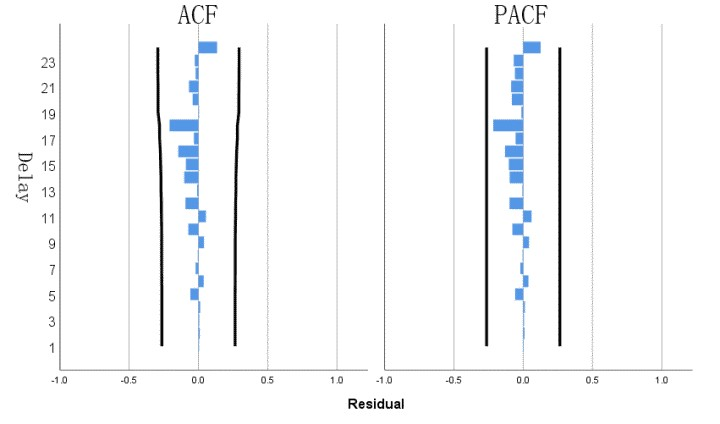
\includegraphics[width = .45\textwidth]{ACF.jpg}
%		\label{sub1}                                        
%	}
%	\qquad
%	\subfloat[Change in Russia`s Population]{                               
%		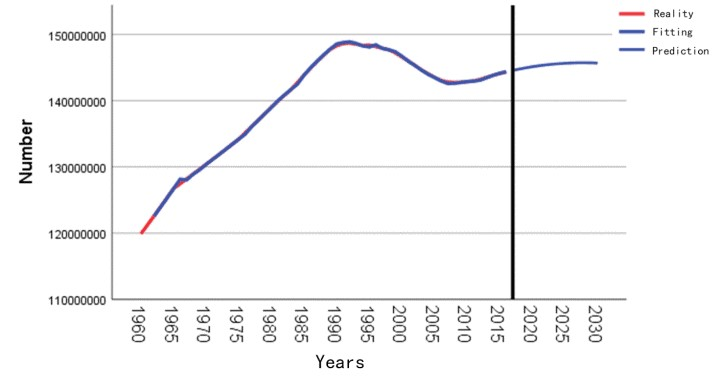
\includegraphics[width = .45\textwidth]{eluosi.jpg}
%		\label{sub2}                                                
%	}\\ 
%	
%	\caption{The Growth Model of Russia`s population}                                      
%	\label{eluosibijiaotu}                                          
%\end{figure}

%\begin{table}[H]
%	\centering
%	\caption{The Change of L1 Speakers in Four Countries}
%	\label{Atu}
%	\begin{tabular}{llllll}
%		\cline{1-3}
%		\multicolumn{1}{c}{}        & \multicolumn{1}{c}{Now} & \multicolumn{1}{c}{In ten years} &  &  &  \\ \cline{1-3}
%		\multicolumn{1}{c}{Russian} & \multicolumn{1}{c}{153} & \multicolumn{1}{c}{162}             &  &  &  \\
%		\multicolumn{1}{c}{English} & \multicolumn{1}{c}{371} & \multicolumn{1}{c}{405}             &  &  &  \\
%		\multicolumn{1}{c}{Chinese} & \multicolumn{1}{c}{897} & \multicolumn{1}{c}{955}             &  &  &  \\
%		\multicolumn{1}{c}{Jpanese} & \multicolumn{1}{c}{128} & \multicolumn{1}{c}{124}             &  &  &  \\ \cline{1-3}
%		
%	\end{tabular}
%\end{table}
%\begin{figure}[H]                                          
%	\centering
%	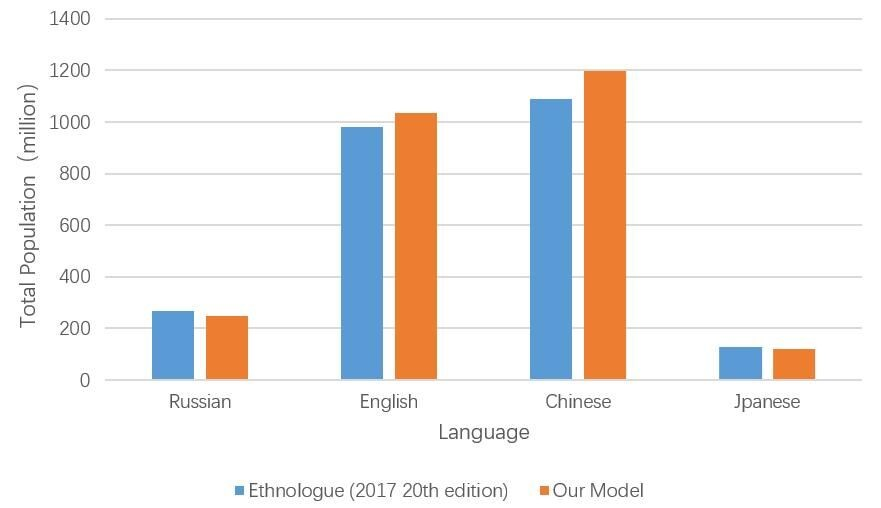
\includegraphics[width = .8\textwidth]{AtuL2.jpg}       
%	\caption{Model Test}                          
%	\label{AtuL2}                                          
%\end{figure}
%
%\begin{table}[H]
%	\centering
%	\caption{The Total Numbers of Four Languages}
%	\label{Bjieguo}
%	\begin{tabular}{cccclcl}
%		\toprule
%		& Native Language      &                      & \multicolumn{2}{c}{Second Language}                     & \multicolumn{2}{c}{Total}                               \\
%		\midrule
%		& Now                  & In Ten Years         & Now                  & \multicolumn{1}{c}{In Ten Years} & Now                  & \multicolumn{1}{c}{In Ten Years} \\
%		Russian              & 153                  & 162                  & 113                  & \multicolumn{1}{c}{119}          & 266                  & \multicolumn{1}{c}{281}          \\
%		English              & 371                  & 405                  & 611                  & \multicolumn{1}{c}{666}          & 982                  & \multicolumn{1}{c}{1071}         \\
%		Chinese              & 897                  & 955                  & 193                  & \multicolumn{1}{c}{205}          & 1090                 & \multicolumn{1}{c}{1160}         \\
%		Jpanese              & 128                  & 124                  & 1                    & \multicolumn{1}{c}{1.2}          & 129                  & \multicolumn{1}{c}{125.2} \\
%		\bottomrule
%	\end{tabular}
%\end{table}


%\begin{table}[H]
%	\centering
%	\caption{The Predictions of 6th-16th Language`s Total Numbers of Speakers}
%	\label{Bdaan}
%	\begin{tabular}{ccccccc}
%		\toprule
%		& \multicolumn{2}{c}{L1} & \multicolumn{2}{c}{L2} & \multicolumn{2}{c}{Total} \\
%		\midrule
%		& Now    & In 50 Years   & Now    & In 50 Years   & Now     & In 50 Years     \\
%		Malay      & 77     & 107           & 204    & 271           & 281     & 378             \\
%		Bengali    & 242    & 340           & 19     & 22            & 261     & 362             \\
%		Russian    & 153    & 183           & 113    & 158           & 267     & 341             \\
%		Portuguese & 218    & 297           & 11     & 16            & 229     & 313             \\
%		French     & 76     & 101           & 153    & 203           & 229     & 304             \\
%		Hausa      & 85     & 132           & 65     & 93            & 150     & 225             \\
%		Punjabi    & 148    & 192           &        &               & 148     & 192             \\
%		German     & 76     & 106           & 52     & 69            & 129     & 175             \\
%		Persian    & 60     & 84            & 61     & 85            & 121     & 169             \\
%		Japanese   & 128    & 164           & 1      & 1.3           & 129     & 165.3           \\
%		Swahili    & 16     & 22            & 91     & 131           & 107     & 153\\
%		\bottomrule
%	\end{tabular}
%\end{table}

\subsection{Solution for Problem Two}
By using Hybrid Algorithm (Take each result of recommendation algorithms into consideration), we can easily get the list of Top 20 Recommended Daters based on sorting the \textbf{Scores} matrix. For acquiring a more suitable estimate of an ideally sized choice set, we can make such an attempt: 
\begin{enumerate}
	\item Divide the users into 20 parts, for i\_th parts, we only recommend i daters, no more or less. 
	\item Gathering the results of dating and do evaluation about the recommendation effect which could be shown as date success rate and user satisfaction degree. 
	\item Do some analysis like regression and correlation on the number of daters and recommendation effect. Then it is clear to see the size of an ideal choice set for most people, which can be seen as large enough to include variety and depth and small enough that someone can fairly weigh each prospect’s potential without tripping his brain’s overload switch. 
	\item Analysis from the difference of character using the same way as step three, for diverse people we can recommend different size of choice set.
\end{enumerate}

%\begin{figure}[H]                                           
%	\centering
%	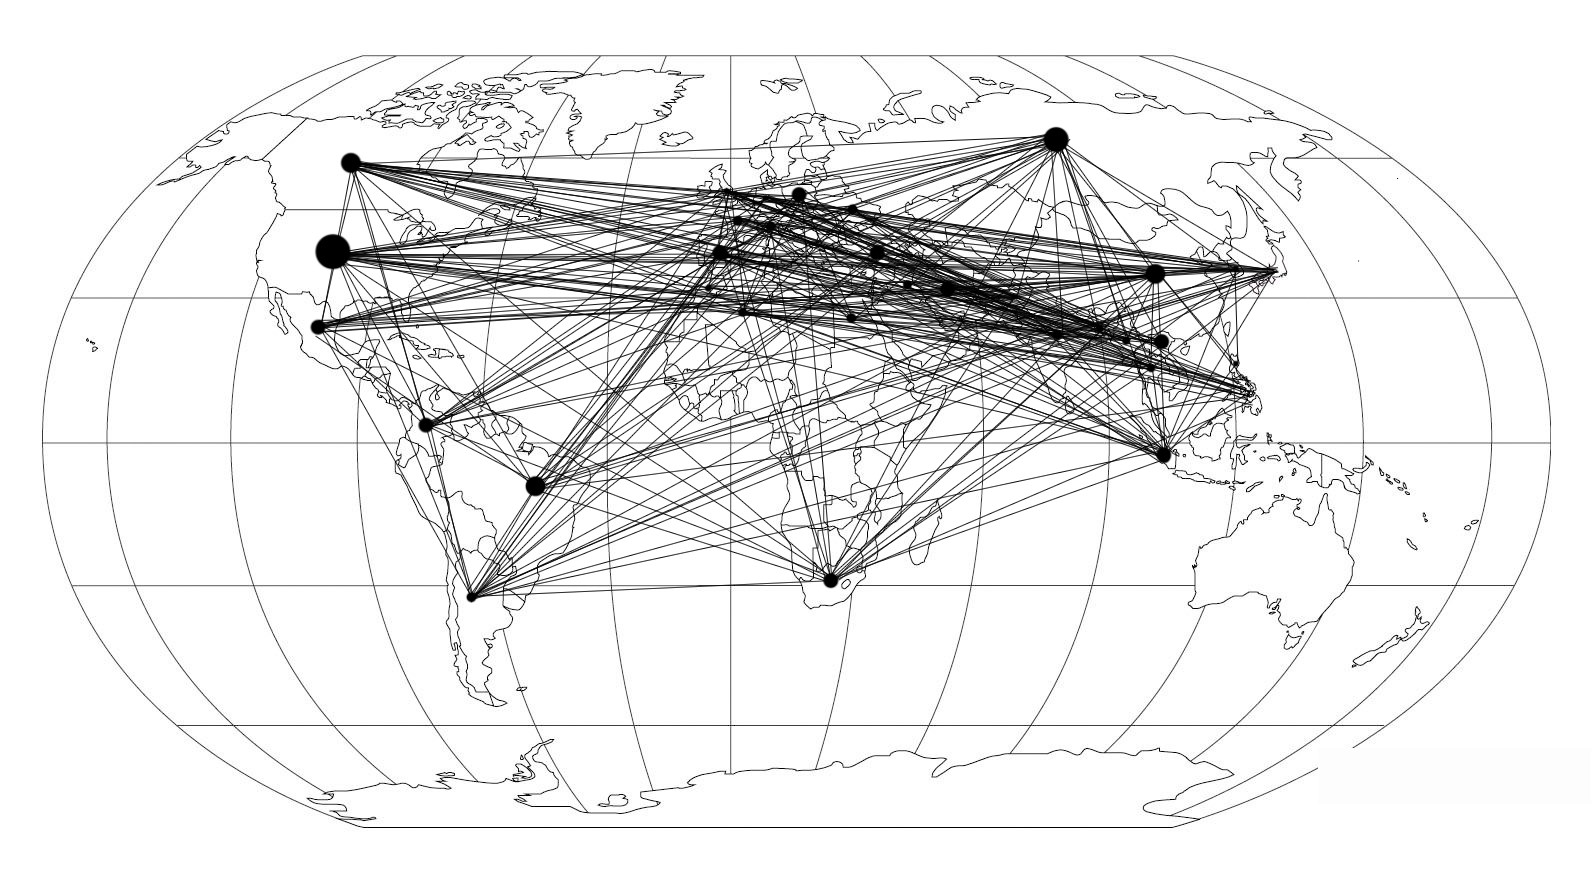
\includegraphics[width = .8\textwidth]{yiduixian.jpg}       
%	\caption{Global Population Mobility Network Space Pattern}                            
%	\label{yiduixian}                                         
%\end{figure}

%\begin{table}[H]
%	\centering
%	\caption{The Different Layer of The Forty Countries}
%	\label{ceng}
%	\begin{tabular}{ccccccclll}
%		\toprule
%		Hierarchy                & \multicolumn{5}{c}{Country}                                   \\
%		\midrule
%		The First Network Layer  & America      & Mexico      & Russian     & Ukraine  & India     \\
%		& Germany      & China       &             &          &          \\
%		\midrule
%		The Second Network Layer & Bangladesh   & Pakistan    & U.K         & France   & Canada    \\
%		& Italy        & Philippines & Iran        &          &           \\
%		\midrule
%		The Third Network Layer  & Turkey       & Spain       & Afghanistan & Algeria  & Poland   \\
%		& Morocco      & Japan       & Viet Nam    & Korea    &           \\
%		\midrule
%		The Forth Network Layer  & Brazil       & Colombia    & Argentina   & Iraq     & Congo   \\
%		& South Africa & Nigeria     & Thailand    & Tanzania & Myanmar   \\
%		& Indonesia    & Sudan       & Egypt       & Kenya    & Uganda   \\
%		& Ethiopia     &             &             &          &          \\
%		\bottomrule
%	\end{tabular}
%\end{table}

\subsection{Solution for Problem Three}
We design a form to collect the necessary information. We use this information to build user profiles and base on this information to recommend dating partner to users.\par 
This information contains five parts:
\begin{itemize}
	\item User's photo: The user must show his face in the photo.
	\item Basic information of the user: For instance, user's name or nickname and so on. See appendix \ref{ap2} for details.
	\item User social attribute information: For instance, user's family number and so on. See appendix \ref{ap2} for details.
	\item Information about ideal dating partner: For instance, the gender of dating partner and so on. See appendix \ref{ap2} for details. 
	\item Information about user character: We design a lot of multiple choice questions to test the user's personality. See appendix \ref{ap2} for details.
\end{itemize}
\par 
In life, when someone ask our what date partner we want to date, we usually use a lot of words to describe the date partner's character. For married people, personality compatibility between husband and wife has a great influence on the quality of marriage\cite{3}. So, we set up a lot of questions to analyze the user's personality in detail.Some domestic research shows that the similarities and differences between couples' character have on significant effect on the quality of marriage. But dissatisfaction with the character of the spouse is an important reason for the decline in the quality of marriage and even thee breakdown of marriage\cite{4}. So, we set up a lot of topics to analyze user preferences. We also set up some questions to get user's basic information, but this information is not the point.\par 
The answers to all questions on the questionnaire can be represented by numbers. So, we can build a matrix to describe the user. The user matrix will be our model's input.\par 
Forms are the basis for collecting information and the primary way to get user information. The quality of the form design has a great influence on the user's portrayal. Inaccurate descriptions of users will greatly affect the accuracy of the model. We create a regression prediction model to solve this problem.\par 
We have designed a total question bank. See appendix \ref{ap2} for details. The questions in the form are form this question bank. We design different forms by changing the number and type of questions in the form. At the same time, calculate the appointment success rate for people using different forms.\par 
We use a column vector to describe a form. Each value of the column vector corresponds to a test question. The total number of rows is the total number of questions in the test question bank. If question A appears in the form, the value which representative question A equal to 1. Else, the value equal to 0. Each form corresponds to a group of people who use the form. We calculate the success rate of dating in this group and think of it as a label for the form.\par
Finally, we group multiple column vectors which represent the forms into a matrix. This matrix is sample set and training data set. Every sample has a corresponding label. We use linear regression in supervised learning to fit the data. The prediction model is: \[f(x;b,w)=w^Tx+b.\] Parameters in prediction is $w \in \mathbb{R}^m$ and $b \in \mathbb{R}$. The input value $x$ is where $ x_j \in \mathbb{R}$ for $ j \in 1,...,m$. $m$ is the number of column vector's row.\par 
After training the model, first predict the label on the training set. After achieving higher accuracy on the training set, using the model, predict dating success rate on form which is not yet in use. At the same time put the form into use. Then, compare the difference between the predicted result and the true value and adjust the model to reduce the gap. When the accuracy of the model is stable at a relatively high level, the model is used to predict the newly designed un-used form, and the form design is adjusted based on the prediction result.\par 
Combine the form and appointment success rate through the model, plus the huge test data of the website, and finally, improve the appointment success rate through high-quality form design.

\subsection{Solution for Problem Four}
Using Data Mining to Match Dating Partner
Data-Mining Dating is a service within the online dating industry to use a scientific approach to matching highly compatible singles. 
Traditional Internet dating can be challening for those singles looking for love that lasts, but Data-Mining Dating is not a traditional dating site. Of all the single men or women you may meet online, very few will be compatible with you specifically, and it can be difficult to determine the level of compatibility of a potential partner through methods of conventional dating services. Our Predict System does the work for you  by narrowing the field from thousands of single prospects to match you with a select group of compatible matches with whom you can build a quality relationship. \par
Our algorithm aims to recommend perfect daters to each user from large crowds. With consideration of all factors you can imagine including personal requests, character matching degree, common outlook on world, life and values and so on, abundant algorithms based on model, content, rules are adopted. In the future, we even will take more factors such as face similarity analysis and gene matching degree into consideration. No best but better and better algorithms will be applied for recommending daters with higher matching degree to you. 

\section{Future Work}
The future work must be using a wider range of algorithms to do online recommendation tests, determining the best  similarity measurement method, and optimizing form design according to the form size-success rate relationship analysis.

\begin{thebibliography}{99}      
	\bibitem{1} Non-profit Organization.Loss function[DB/OL].(2018-10-02)[2018-12-02].https://en.  \\ wikipedia.org/wiki/Loss\_function    
	\bibitem{2} MuShi.Machine Learning: Comparisons of Several Distance Metrics[EB/OL].(2016-11-14)[2018-12-02].https://my.oschina.net/hunglish/blog/787596     
	 \bibitem{3} CHENG Zao-Huo, TAN Lin-Xiang, ZHAO Yong, et al. Spouse's Personality and Marital Quality[J]. Chinese Mental Health Journal, 2006, 20 (4): 268-271
	\bibitem{4} Li Ling-Jiang, Yang De-Sen. A control study on the personality of 100 couples in divorce proceedings[J]. Chinese Mental Health Journal, 1993, 007 (2):70-72
\end{thebibliography}

\begin{appendices}

	
	\section{Model 1: k-means -- example on iris data set \label{apA}}
    \begin{lstlisting}[language=python]	
	
	from sklearn.datasets import load_iris
	import matplotlib.pyplot as plt
	from numpy import *
	
	iris = load_iris() 
	data=iris['data']
	target=iris['target']
	X=data
	Y=target
	def calDistance(centroid, point):
	return sqrt(sum(power(centroid-point,2)))
	
	def constructCentroidSet(dataSet,K):
	numOfCoordinate = dataSet.shape[1]
	
	centroidSet=mat(zeros((K,numOfCoordinate)))

	for ith_coordinate in range(numOfCoordinate):  
	min_ith_coordinate=min(dataSet[:,ith_coordinate])
	max_ith_coordinate=max(dataSet[:,ith_coordinate])
	range_coordinate=max_ith_coordinate-min_ith_coordinate  
	centroidSet[:,ith_coordinate] = min_ith_coordinate+range_coordinate* \
	random.rand(K,1)
	return centroidSet
	
	def kMeans(dataSet, k):
	numOfsamples= dataSet.shape[0]  
	
	class_distance = mat(zeros((numOfsamples,2)))   
	centroidSet = constructCentroidSet(dataSet, k)
	NoChangeHappened = False  
	
	while not NoChangeHappened:
	NoChangeHappened = True;
	for ith_sample in range(numOfsamples): 
	minDistance = inf 
	classIndex = -1     
	for jth_cluster in range(k):
	distance_ith_sample_jth_cluster = calDistance(centroidSet[jth_cluster,:], \
	 dataSet[ith_sample,:])

	if distance_ith_sample_jth_cluster < minDistance:
	minDistance = distance_ith_sample_jth_cluster
	classIndex = jth_cluster
	
	if class_distance[ith_sample,0] != classIndex: 
	NoChangeHappened = False  
	class_distance[ith_sample,:] = classIndex , minDistance 
	
	for ith_centroid in range(k):   
	class_row_isCentroid= nonzero(class_distance[:,0].A==ith_centroid)[0]      
	sample_is_centroid = dataSet[class_row_isCentroid]   
	
	centroidSet[ith_centroid,:] = mean(sample_is_centroid, axis = 0)  
	#print(centroidSet)
	
	return centroidSet, class_distance
	

	def getClassValue(aclass):
	for i in aclass:
	return argmax(bincount(i))

	
	accuracies=[]
	run_times=300 
	for test_times in range(run_times):
	
	centroids,class_distance=kMeans(data,3)
	#print(class_distance)
	#print(centroidSet)
	
	
	class1=(array(class_distance[0:50,0]).T).astype(int)
	class2=(array(class_distance[50:100,0]).T).astype(int)
	class3=(array(class_distance[100:150,0]).T).astype(int)

	class1_name=getClassValue(class1)
	class2_name=getClassValue(class2) 
	class3_name=getClassValue(class3) 
	#print('class1: ',class1_name,'class2: ',class2_name,'class3: ',class3_name)
	
	accuracy=0
	accuracy= (sum(class1==class1_name)+sum(class2==class2_name)+ \
	sum(class3==class3_name))/150
	print(accuracy)
	accuracies.append(accuracy)
	print("average accuracy: ")
	print(sum(accuracies)/run_times)

	
	%matplotlib inline
	import matplotlib.pyplot as plt
	
	plt.figure(figsize=(18,10))
	plt.plot(accuracies, "-", color="black", label="accuracy")
	plt.xlabel("run_times")
	plt.ylabel("accuracy")
	plt.legend() 
	plt.title("kMeans")
	
	\end{lstlisting}
    \section{Model 2: KNN -- example on iris data set \label{apB}}
    \begin{lstlisting}[language=python]
    import pandas as pd
    import numpy as np
    
    class kNN:
    def __init__(self,X,y,split=0.2,test='YES'):
    
    if isinstance(X,pd.core.frame.DataFrame) != True:  
    self.X = pd.DataFrame(X)
    else:
    self.X = X
    if isinstance(y,pd.core.series.Series) != True:
    self.y = pd.Series(y)
    else:
    self.y = y  
    
    self.max_data = np.max(self.X,axis=0)
    self.min_data = np.min(self.X,axis=0)
    max_set = np.zeros_like(self.X); max_set[:] = self.max_data 
    min_set = np.zeros_like(self.X); min_set[:] = self.min_data
    self.X = (self.X - min_set)/(max_set - min_set)
    
  
    if test == 'YES':     
    self.test = 'YES'   
    n_samples = len(self.X)
    trainDataSet = [i for i in range(n_samples)]  # 0-149
    testSet = []                          
    for i in range(int(n_samples*split)):
    random_num = trainDataSet[int(np.random.uniform(0,len(trainDataSet)))]
    testSet.append(random_num) 
    trainDataSet.remove(random_num)
    self.X,self.testSet_X = self.X.iloc[trainDataSet],self.X.iloc[testSet]
    self.y,self.testSet_y = self.y.iloc[trainDataSet],self.y.iloc[testSet]
    else:
    self.test = 'NO'
    
    def getDistances(self,point):  
    points = np.zeros_like(self.X)   
    points[:] = point                
    minusSquare = (self.X - points)**2  
    EuclideanDistances = np.sqrt(minusSquare.sum(axis=1)) 
    return EuclideanDistances
    
    
    def getClass(self,point,k):    
    distances = self.getDistances(point)
    argsort = distances.argsort(axis=0)       
    classList = list(self.y.iloc[argsort[0:k]])
    classCount = {}
  
    for i in classList:
    if i not in classCount:
    classCount[i] = 1
    else:
    classCount[i] += 1
    maxCount = 0
    maxkey = 'x'
    for key in classCount.keys():
    if classCount[key] > maxCount:
    maxCount = classCount[key]
    maxkey = key
    return maxkey
    
    
    def knn(self,testData,k):     
    if self.test == 'NO':    
    testData = pd.DataFrame(testData)
    max_set = np.zeros_like(testData); max_set[:] = self.max_data
    min_set = np.zeros_like(testData); min_set[:] = self.min_data
    testData = (testData - min_set)/(max_set - min_set)   
    if testData.shape == (len(testData),1): 
    label = self.getClass(testData.iloc[0],k)
    return label                      
    else:
    labels = []
    for i in range(len(testData)):
    point = testData.iloc[i,:]
    label = self.getClass(point,k)
    labels.append(label)
    return labels                    
    
    
    def errorRate(self,knn_class,real_class):   
    error = 0
    allCount = len(real_class)
    real_class = list(real_class)
    for i in range(allCount):
    if knn_class[i] != real_class[i]:
    error += 1
    return error/allCount
    \end{lstlisting}

	\section{Information Forms Design \label{ap2}}
		
		\begin{itemize}
		\item User basic information:
		\begin{enumerate}
			\item name/nickname
			\item I am a man/woman.
			\item How many children do you have?
			\item When were you born?
			\item Where do you live?
			\item What is your nation?
			\begin{itemize}
				\item white
				\item Hispanic/Latino
				\item black/African descent
				\item Asian/pacific islander
				\item Indian
				\item Chinese			
				\item native American
				\item Arabic/middle eastern
				\item Korean
				\item Japanese
				\item other
			\end{itemize}
			\item What best describes your religious beliefs or spirituality?
			\begin{itemize}
				\item christian
				\item Jewish
				\item Muslim
				\item Hindu
				\item Buddhist
				\item Sikh
				\item Shinto
				\item other
				\item spiritual
				\item but not religious
				\item neither religious nor spiritual
				\item Baha'i
				\item cao dai
				\item Confucianism
				\item Jainism
				\item christian science
				\item Rastafarianism
				\item Taoism
				\item Tokyoite
				\item Unitarian-universalism
				\item Scientology
				\item metaphysical
				\item pagan
				\item Wiccan
				\item new age
				\item prefer not to specify 
			\end{itemize}  
			\item Which describes your highest level of education?
			\begin{itemize}
				\item doctorate
				\item masters
				\item bachelors
				\item associates
				\item some college
				\item high school
			\end{itemize} 
			\item What is you job?
			\item What's your personal income?(Your matches won't see this.)
			\item How often do you smoke?
			\begin{itemize}
				\item never
				\item socially
				\item once a week
				\item few times a week
				\item daily
			\end{itemize}
			\item How often do you drink?
			\begin{itemize}
				\item never
				\item on special occasions
				\item once a week
				\item few times a week
				\item daily
			\end{itemize}
			\item How tall are you?
			\item What are you passionate about?
			\item What two or three things do you enjoy doing with you leisure time?
		\end{enumerate}
		\item User social attribute information.(Optional)
		\begin{enumerate}
			\item Family members
			\item Graduated school
		\end{enumerate}
		\item Information about ideal dating partner.
		\begin{enumerate}
			\item I am seeking a man/woman.
			\item I am looking for someone between the ages of xx-xx.
			\item How far should we search for your matches?  x miles.
			\item How important is the distance of your match?
			\begin{itemize}
				\item not at all important
				\item somewhat important
				\item very important
			\end{itemize}
		\end{enumerate}
		\item Information about user character.
		\begin{enumerate}
			\item How well dose this generally describe you?(Not at all / somewhat / very well)
			\begin{itemize}
				\item warm
				\item clever
				\item dominant
				\item outgoing
				\item quarrelsome
				\item stable
				\item energetic
				\item predictable
				\item affectionate
				\item intelligent
				\item attractive
				\item compassionate
				\item loyal
				\item witty
				\item sensitive
				\item generous
				\item sensual
				\item stylish			
				\item athletic
				\item overweight
				\item plain
				\item healthy
				\item sexy
				\item content
				\item patient
				\item passionate
				\item caring
				\item genuine
				\item vivacious
				\item wise
				\item bossy
				\item leader
				\item irritable
				\item kind
				\item aggressive
				\item outspoken
				\item opinionated
				\item restless
				\item romantic
				\item selfish
				\item stubborn
				\item I do things according to a plan.
				\item I take time out for others.
				\item I feel unable to deal with things.
				\item I love to help others.
				\item I seek adventure.
				\item I desire sexual activity.
				\item I often leave a mess in my room.
				\item I often carry the conversation to a higher level.
				\item I get stressed out easily.
				\item I often make others feel good.
				\item I am good at analyzing problems.
				\item I usually stand up for myself.
				\item I am easily discouraged.
				\item I can handle a lot of information.
				\item I waste my time.
				\item I catch on quickly.
				\item I usually wait for others to lead the way.
				\item I love order and regularity.
				\item I often do nice things for people.
				\item I get angry easily.
				\item My personal religious beliefs are important.
				\item I ask questions in search of information.
				\item I think it is important to continually try to improve myself.
				\item I care about the physical shape I'm in.
				\item I feel better when I am around other people.
				\item I try to accommodate the other person's position.
				\item I try to understand the other person.
				\item I try to be respectful of all opinions different from my own.
				\item I try to resolve conflict well.
			\end{itemize}
			\item How strongly do you agree or disagree with...?(Absolutely disagree / Neither agree nor disagree / Absolutely agree)
			\begin{itemize}
				\item I am looking for a long-term relationship that will ultimately lead to marriage.
				\item When I get romantically involved, I tell my partner just about everything.
				\item It is difficult for me to let people get emotionally close to me.
				\item A "serious" relationship needs to be exclusive (i.e. monogamous).
				\item I know I can always count on the people who are closest to me.
				\item I don't need to have close relationships to be happy.
				\item Being monogamous helps build intimacy and trust in a romantic relationship.
				\item People often let you down if you depend on them.
				\item It's important for me to have close friends in my life.
				\item Being exclusive (i.e., monogamous) is one of benefits of being in a successful relationship.
				\item I sometimes find it difficult to trust people I get romantically involved with.
				\item I find it easy to get emotionally close to people.		
			\end{itemize}
			\item How important in a relationship is...(Not at all important / Somewhat important / Very important)
			\begin{itemize}
				\item My partner's dependability.
				\item My partner's sex appeal.
				\item My partner's physical appearance.
				\item Enjoying the way I feel around my partner.
				\item Our sexual compatibility.
				\item The friendship between me and my partner.
				\item Enjoying physical closeness with my partner.
				\item Being able to spend as much time as possible with my partner.
				\item Doing special things to let my partner know how important he/she is to me.
			\end{itemize}
			\item How happy are you with your physical appearance?
			\begin{itemize}
				\item Not at all
				\item Somewhat happy
				\item Very happy
			\end{itemize}
			\item How often in the past month have you felt...?(Really / Occasionally / Almost Always)
			\begin{itemize}
				\item Happy
				\item Sad
				\item Anxious
				\item Confident
				\item Hopeful
				\item Fearful about future
				\item Angry
				\item Calm
				\item Fortunate
				\item Out of control
				\item Fulfilled
				\item Depressed
				\item Unable to cope
				\item Satisfied
				\item Misunderstood
				\item Plotted against			
			\end{itemize}
			\item How skilled you are at the following things:(Not skilled / Somewhat Skilled / Very Skilled)
			\begin{itemize}
				\item Creating romance in a relationship
				\item Keeping physically fit
				\item Finding and taking on challenging activities
			\end{itemize}
			\item What's your interest in....?(None / Some Interest / Very Strong Interest)
			\begin{itemize}
				\item Watching movies
				\item Listening to music
				\item Watching TV
				\item Reading
				\item Parties
				\item Dining out
				\item Traveling
				\item Shopping
				\item Family
				\item Talking with friends
				\item Religious Community
				\item Religious Faith
				\item Conversation
				\item Hosting/Entertaining
				\item Church Involvement
			\end{itemize}
			\item If your best friends had to pick four words to describe you, which four from this list would they pick?
			\begin{itemize}
				\item good listener 
				\item modest
				\item respectful
				\item affectionate
				\item caring
				\item spontaneous
				\item physically
				\item fit
				\item warm
				\item outgoing
				\item optimistic
				\item dependable
				\item romantic
				\item creative
				\item loyal
				\item spiritual
				\item kind
				\item ambitious
				\item articulate
				\item rational
				\item easy-going
				\item generous
				\item happy
				\item quiet
				\item genuine
				\item intelligent
				\item sweet
				\item passionate
				\item energetic
				\item funny
				\item perceptive
			\end{itemize}
		\end{enumerate}
	\end{itemize}

\end{appendices}
